\documentclass[a4paper, 14pt]{extarticle}

% Поля
%--------------------------------------
\usepackage{geometry}
\geometry{a4paper,tmargin=2cm,bmargin=2cm,lmargin=3cm,rmargin=1cm}
%--------------------------------------


%Russian-specific packages
%--------------------------------------
\usepackage[T2A]{fontenc}
\usepackage[utf8]{inputenc}
\usepackage[english, main=russian]{babel}
\usepackage{cmap}
%--------------------------------------

\usepackage{textcomp}
\usepackage{amssymb}

% Красная строка
%--------------------------------------
\usepackage{indentfirst}               
%--------------------------------------             


%Graphics
%--------------------------------------
\usepackage{graphicx}
\graphicspath{ {./images/} }
\usepackage{wrapfig}
%--------------------------------------

% Полуторный интервал
%--------------------------------------
\linespread{1.3}                    
%--------------------------------------

%Выравнивание и переносы
%--------------------------------------
% Избавляемся от переполнений
\sloppy
% Запрещаем разрыв страницы после первой строки абзаца
\clubpenalty=10000
% Запрещаем разрыв страницы после последней строки абзаца
\widowpenalty=10000
%--------------------------------------

%Списки
\usepackage{enumitem}

%Подписи
\usepackage{caption} 

%Гиперссылки
\usepackage{hyperref}

\hypersetup {
	unicode=true
}

%Рисунки
%--------------------------------------
\DeclareCaptionLabelSeparator*{emdash}{~--- }
\captionsetup[figure]{labelsep=emdash,font=onehalfspacing,position=bottom}
%--------------------------------------

\usepackage{tempora}
\usepackage{amsmath}
\usepackage[dvipsnames]{xcolor}
\usepackage{listings}
\lstset{
  belowcaptionskip=1\baselineskip,
  breaklines=true,
  frame=L,
  xleftmargin=\parindent,
  language=Java,
  showstringspaces=false,
  basicstyle=\footnotesize\ttfamily,
  keywordstyle=\bfseries\color{blue},
  commentstyle=\itshape\color{purple},
  identifierstyle=\color{black},
  stringstyle=\color{red},
  numbers=left,           
  numberstyle=\tiny\color{gray}, 
  numbersep=10pt,      
  % ------------------------------
}

%--------------------------------------
%			НАЧАЛО ДОКУМЕНТА
%--------------------------------------

\begin{document}

%--------------------------------------
%			ТИТУЛЬНЫЙ ЛИСТ
%--------------------------------------
\begin{titlepage}
\thispagestyle{empty}
\newpage


%Шапка титульного листа
%--------------------------------------
\vspace*{-60pt}
\hspace{-65pt}
\begin{minipage}{0.3\textwidth}
\hspace*{-20pt}\centering

\includegraphics[width=\textwidth]{emblem}
\end{minipage}
\begin{minipage}{0.67\textwidth}\small \textbf{
\vspace*{-0.7ex}
\hspace*{-6pt}\centerline{Министерство науки и высшего образования Российской Федерации}
\vspace*{-0.7ex}
\centerline{Федеральное государственное бюджетное образовательное учреждение }
\vspace*{-0.7ex}
\centerline{высшего образования}
\vspace*{-0.7ex}
\centerline{<<Московский государственный технический университет}
\vspace*{-0.7ex}
\centerline{имени Н.Э. Баумана}
\vspace*{-0.7ex}
\centerline{(национальный исследовательский университет)>>}
\vspace*{-0.7ex}
\centerline{(МГТУ им. Н.Э. Баумана)}}
\end{minipage}
%--------------------------------------

%Полосы
%--------------------------------------
\vspace{-25pt}
\hspace{-35pt}\rule{\textwidth}{2.3pt}

\vspace*{-20.3pt}
\hspace{-35pt}\rule{\textwidth}{0.4pt}
%--------------------------------------

\vspace{1.5ex}
\hspace{-35pt} \noindent \small ФАКУЛЬТЕТ\hspace{80pt} <<Информатика и системы управления>>

\vspace*{-16pt}
\hspace{47pt}\rule{0.83\textwidth}{0.4pt}

\vspace{0.5ex}
\hspace{-35pt} \noindent \small КАФЕДРА\hspace{50pt} <<Теоретическая информатика и компьютерные технологии>>

\vspace*{-16pt}
\hspace{30pt}\rule{0.866\textwidth}{0.4pt}
  
\vspace{11em}

\begin{center}
\Large {\bf Лабораторная работа № 5} \\ 
\large {\bf по курсу <<Языки и методы программирования>>} \\ 
\large <<Монады в языке Java>>
\end{center}\normalsize

\vspace{8em}


\begin{flushright}
  {Студент группы ИУ9-21Б Воронков А. С.\hspace*{15pt} \\
  \vspace{2ex}
  Преподаватель Посевин Д. П.\hspace*{15pt}}
\end{flushright}

\bigskip

\vfill
 

\begin{center}
\textsl{Москва 2026}
\end{center}
\end{titlepage}
%--------------------------------------
%		КОНЕЦ ТИТУЛЬНОГО ЛИСТА
%--------------------------------------

\renewcommand{\ttdefault}{pcr}

\setlength{\tabcolsep}{3pt}
\newpage
\setcounter{page}{2}

\section{Цель}\label{Sect::task}
\par 
Приобретение навыков использования монад Optional и Stream в программах на языке 
Java.    
\section{Задание}
В течение лабораторной работы нужно реализовать следующие классы:
\begin{itemize}
    \item Множество целых чисел, представленных объектами класса BigInteger, с операциями: 
\begin{itemize}
    \item Порождение потока таких чисел последовательности, что десятичное представление каждого из них содержит все возможные цифры; 
    \item Поиск максимального числа с максимальной суммой составляющих его десятичное представление цифр.
\end{itemize}

Проверить работу второй операции нужно путём ранжирования чисел потока по длине их десятичного представления. 

 
    \item Булевская матрица размером m × n, где $1 \leq m$, $n \leq 8$, с операциями: 
\begin{itemize}
    \item Порождение потока сумм элементов строк по модулю 2 (т.е., исключающее ИЛИ); 
    \item Поиск строки, в которой единиц больше, чем во всех остальных строках вместе взятых. Элементы матрицы должны быть представлены битами в числе типа long. 
\end{itemize}

Проверить работу первой операции нужно путём подсчёта количества нулевых и ненулевых сумм. 



\end{itemize}

\pagebreak
\section{Практическая реализация}
\par
Код файла Test.java
\begin{lstlisting}
import javax.swing.text.html.Option;
import java.math.BigInteger;
import java.util.*;
import java.util.stream.Stream;
import java.util.stream.Collectors;

class IntsStream {
    ArrayList<BigInteger> Ints;
    IntsStream() {
        Ints = new ArrayList<>();
    }
    void add(BigInteger i) {
        Ints.add(i);
    }

    boolean isAllDig(String s) {
        String digits = "0123456789";
        for (char d : digits.toCharArray()) {
            if (s.indexOf(d) == -1) {
                return false;
            }
        }
        return true;
    }
    public Stream<BigInteger> nameStream() {
        return Ints.stream()
                .filter(x -> isAllDig(x.toString()));
    }
    public Optional<BigInteger> getInt() {
        return Ints.stream()
                .max(new SumComparator());
    }
}
class SumComparator implements Comparator<BigInteger> {
    int SumDigs(BigInteger s) {
        int sm = 0;
        for (char d : s.toString().toCharArray()) {
            sm += Character.getNumericValue(d);
        }
        return sm;
    }

    public int compare(BigInteger a, BigInteger b) {
        int a0 = SumDigs(a);
        int b0 = SumDigs(b);
        if (a0 > b0) { return 1; }
        if (a0 == b0) { return a.compareTo(b);}
        return -1;
    }
}
public class Test {
    public static void main(String[] args) {
        IntsStream t = new IntsStream();
        t.add(new BigInteger("4258178233903402576"));
        t.add(new BigInteger("4930125084"));
        t.add(new BigInteger("1234567890"));
        t.add(new BigInteger("9349200238577294423757"));
        t.nameStream().forEach(System.out::println);
        Map<Integer, List<BigInteger>> groupedByLength = t.Ints.stream()
                .collect(Collectors.groupingBy(x -> x.toString().length()));
        groupedByLength.forEach((len, list) -> {
            BigInteger maxInGroup = list.stream().max(new SumComparator()).get();
            System.out.println("len " + len + " digits: max for sum = " + maxInGroup);
        });

        System.out.println("summary max: " + t.getInt().orElse(BigInteger.ZERO));
    }
}
\end{lstlisting}
\par
Код файла Test2.java
\begin{lstlisting}
import java.util.Optional;
import java.util.*;
import java.util.stream.Stream;
import java.util.stream.IntStream;
import java.util.stream.Collectors;

class Matrix {
    public long matrix;
    public int m, n;
    Matrix(long matrix, int m, int n) {
        this.matrix = matrix;
        this.m = m;
        this.n = n;
    }
}

class MatrixStream {
    Matrix matrix;
    long mask;
    int total;
    MatrixStream(long num, int m, int n) {
        this.matrix = new Matrix(num, m, n);
        this.mask = (1L << matrix.n) - 1;
        this.total = Long.bitCount(matrix.matrix);
    }

    public Stream<Integer> MatStream() {
        return IntStream.range(0, matrix.m)
                .mapToObj(i -> Long.bitCount(matrix.matrix >> (i * matrix.n) & mask) % 2);
    }
    public Optional<Integer> getMaxOnes() {
        return IntStream.range(0, matrix.m)
                .filter(i -> 2 * Long.bitCount(matrix.matrix >> (i * matrix.n) & mask) > total)
                .boxed()
                .findFirst();
    }
}

public class Test2 {
    public static void main(String[] args) {
        long num = Long.parseLong("0000" + "0001" + "1111", 2);

        MatrixStream t = new MatrixStream(num, 3, 4);
        Map<Integer, Long> check = t.MatStream()
                .collect(Collectors.groupingBy(s -> s, Collectors.counting()));
        System.out.println("zero sum: " + check.getOrDefault(0, 0L));
        System.out.println("nonzero sum: " + check.getOrDefault(1, 0L));
        t.getMaxOnes().ifPresent(System.out::println);
    }
}
\end{lstlisting}

\section{Результаты}
В результате лабораторной работы были созданы классы множеств целых чисел и булевых матриц с соответствующими операциями

\begin{center}
    \nopagebreak
    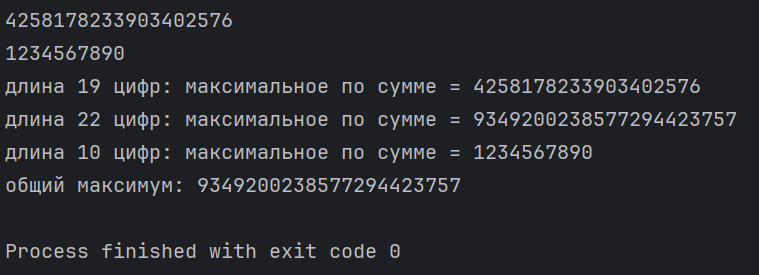
\includegraphics[width=0.85\textwidth]{lab5_1}
    \captionsetup{justification=centering}
    \captionof{figure}{Класс множеств целых чисел}
    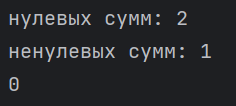
\includegraphics[width=0.85\textwidth]{lab5_2}
    \captionsetup{justification=centering}
    \captionof{figure}{Класс булевых матриц}
\end{center}

\section{Вывод}
В данной лабораторной работе были получены навыки работы с монадами Stream и Optional
\end{document}